\newpage
\section{Interface design process}\label{apdx:design}
In this section, we outline the design process leading to our final interface.% As mentioned in the paper, our design iteration began from existing QV applications in the wild.

\begin{figure}[H]
    \centering
    % First subfigure
    \begin{subfigure}[b]{\linewidth}
        \centering
        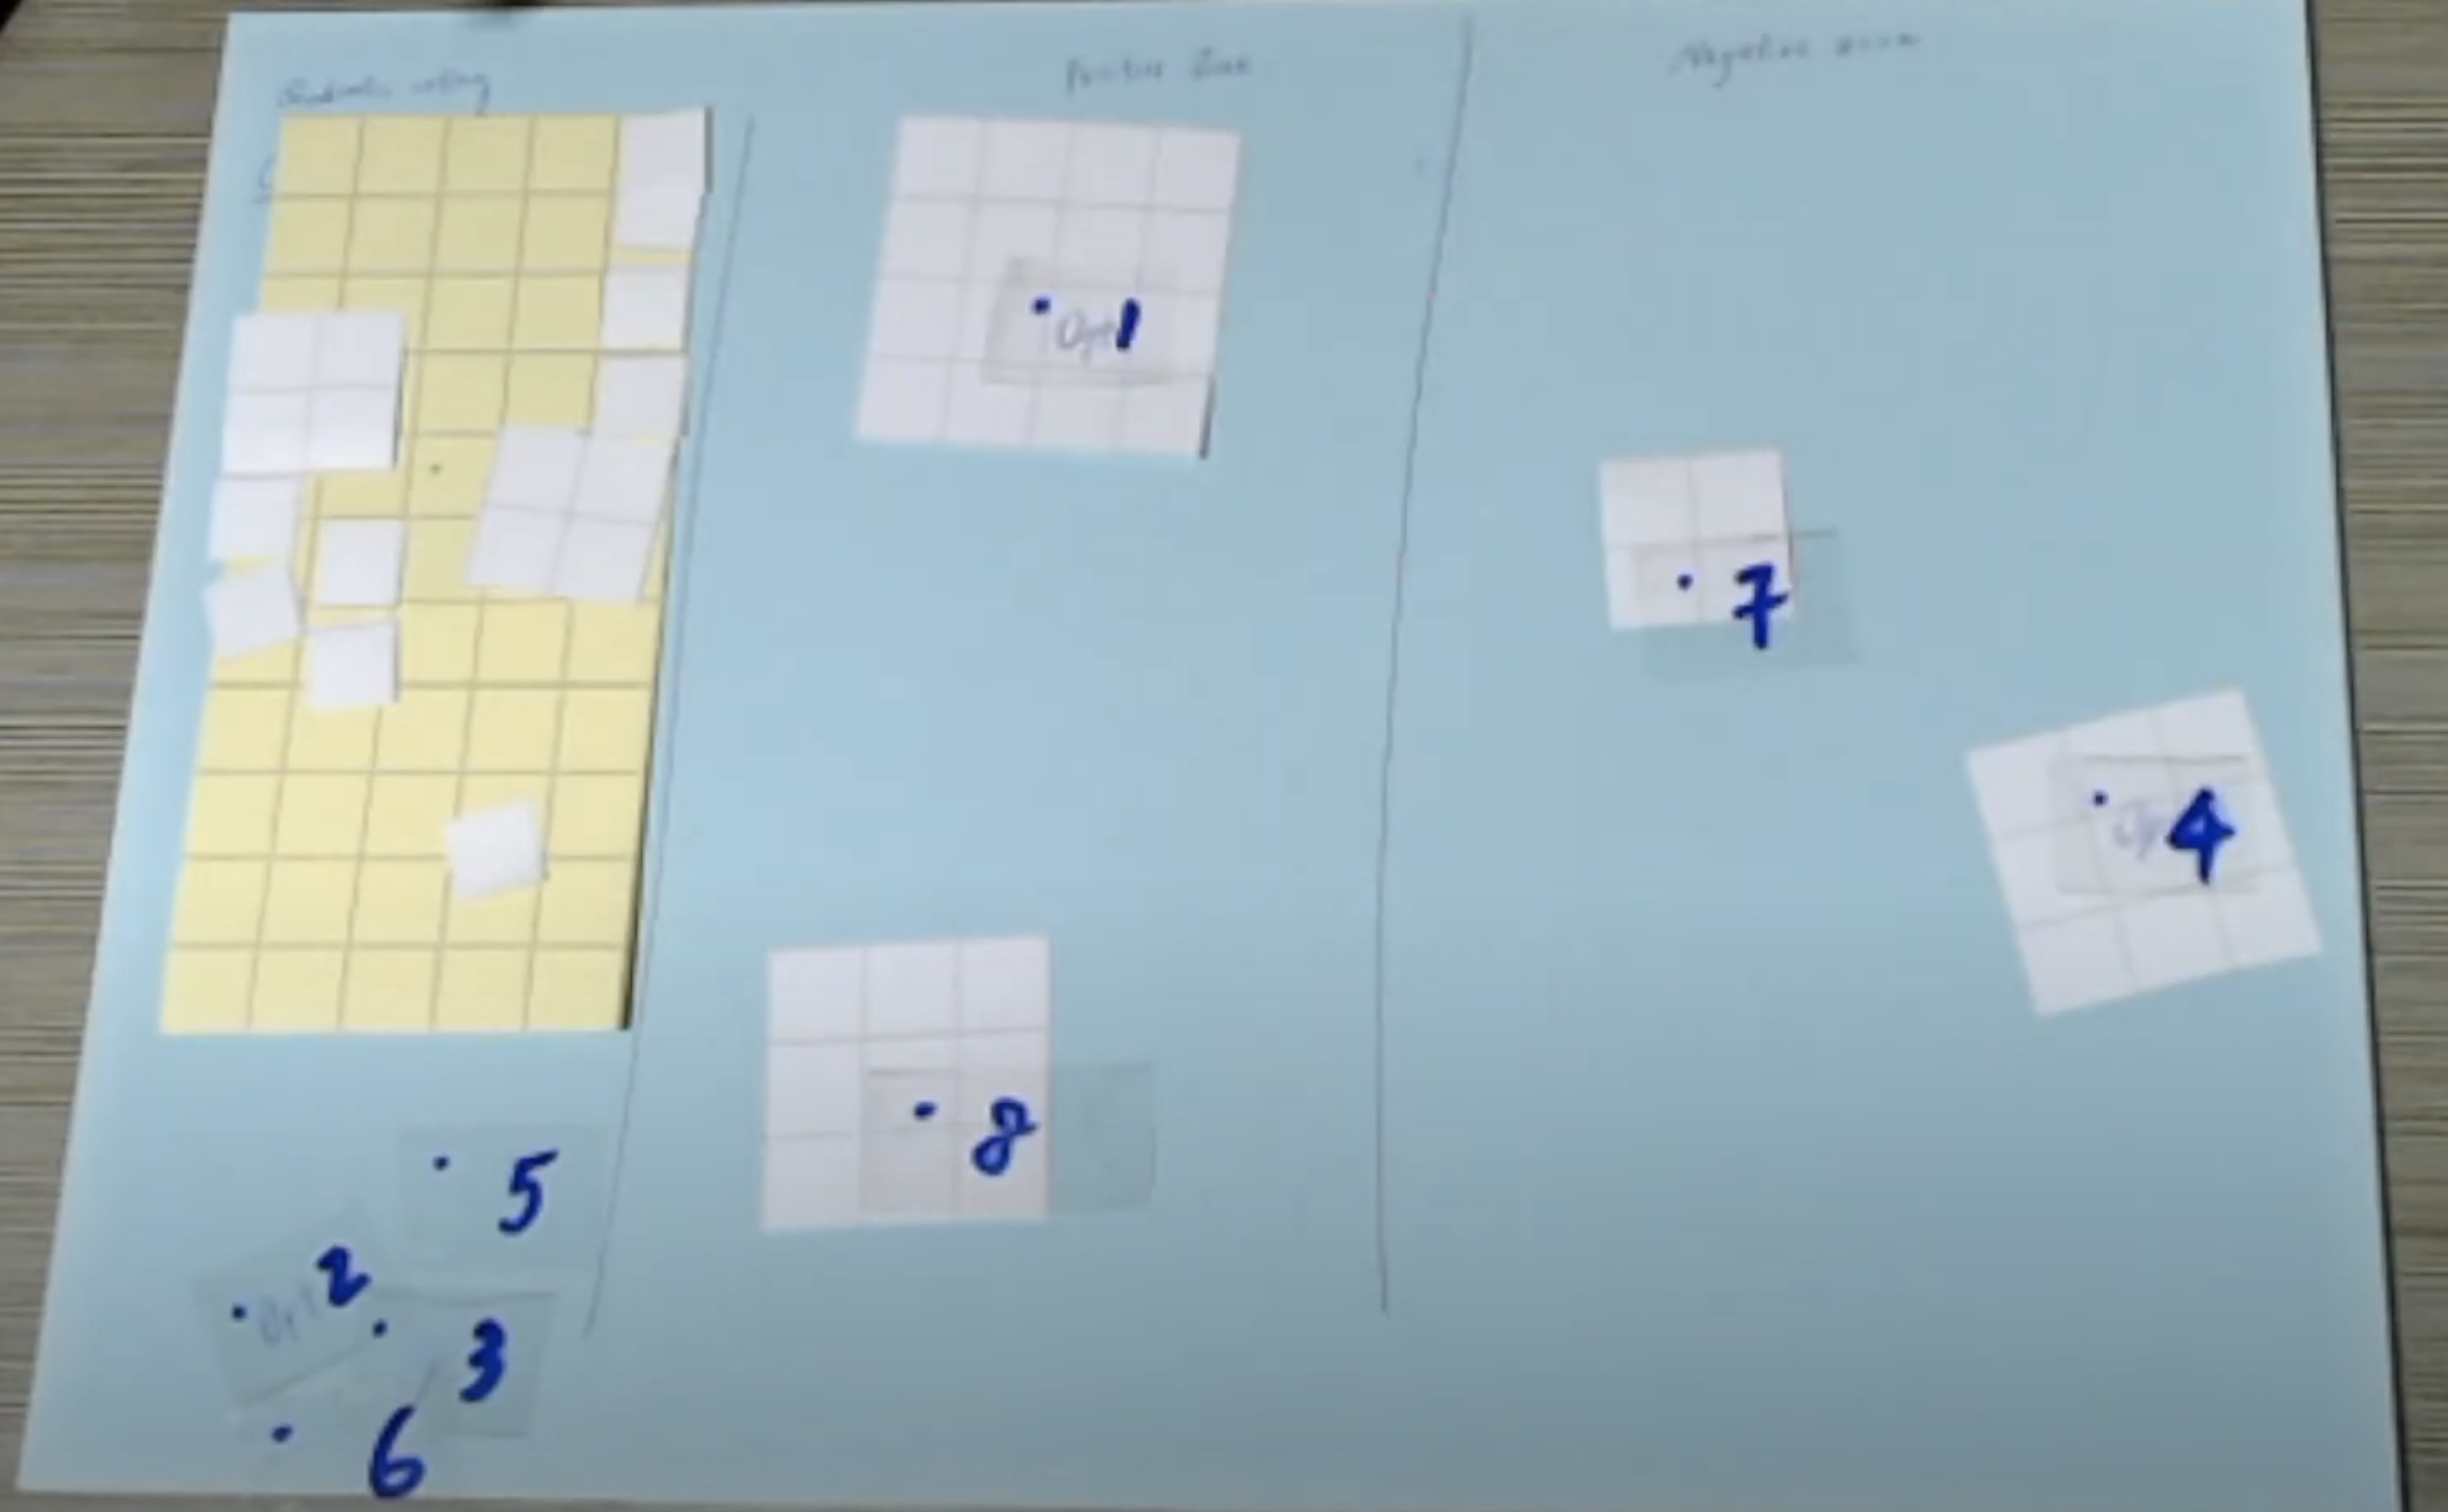
\includegraphics[width=0.9\linewidth]{content/image/prototypes/1.2_paper_qv_single.png}
        \caption{In this paper prototype, issues are denoted by different numbers that appear on mouseover. Pretest respondents can move options anywhere in the two sections of the interface, one denoting positive and one negative. The blocks represent the cost for each option, with no indication of the number of current votes. The credits are shown in the yellow box on the left.}
        \Description{An image of a paper prototype showing different sections for respondents to interact with. On the left side, a yellow grid contains small white squares, some of which are stacked and scattered outside the grid. The middle section labeled "Positive Zone" contains a large white square with a grid, labeled "Opt 1". The right section, labeled "Negative Zone," contains two white squares, each with grids, labeled with numbers 7 and 4. Additional small white squares labeled with numbers 2, 3, 5, 6, and 8 are positioned around the prototype. The yellow box on the left represents available credits.}
        \label{fig:horizontal_paper}
    \end{subfigure}

    \vspace{1em} % Adjusts vertical spacing between figures

    % Second subfigure
    \begin{subfigure}[b]{\linewidth}
        \centering
        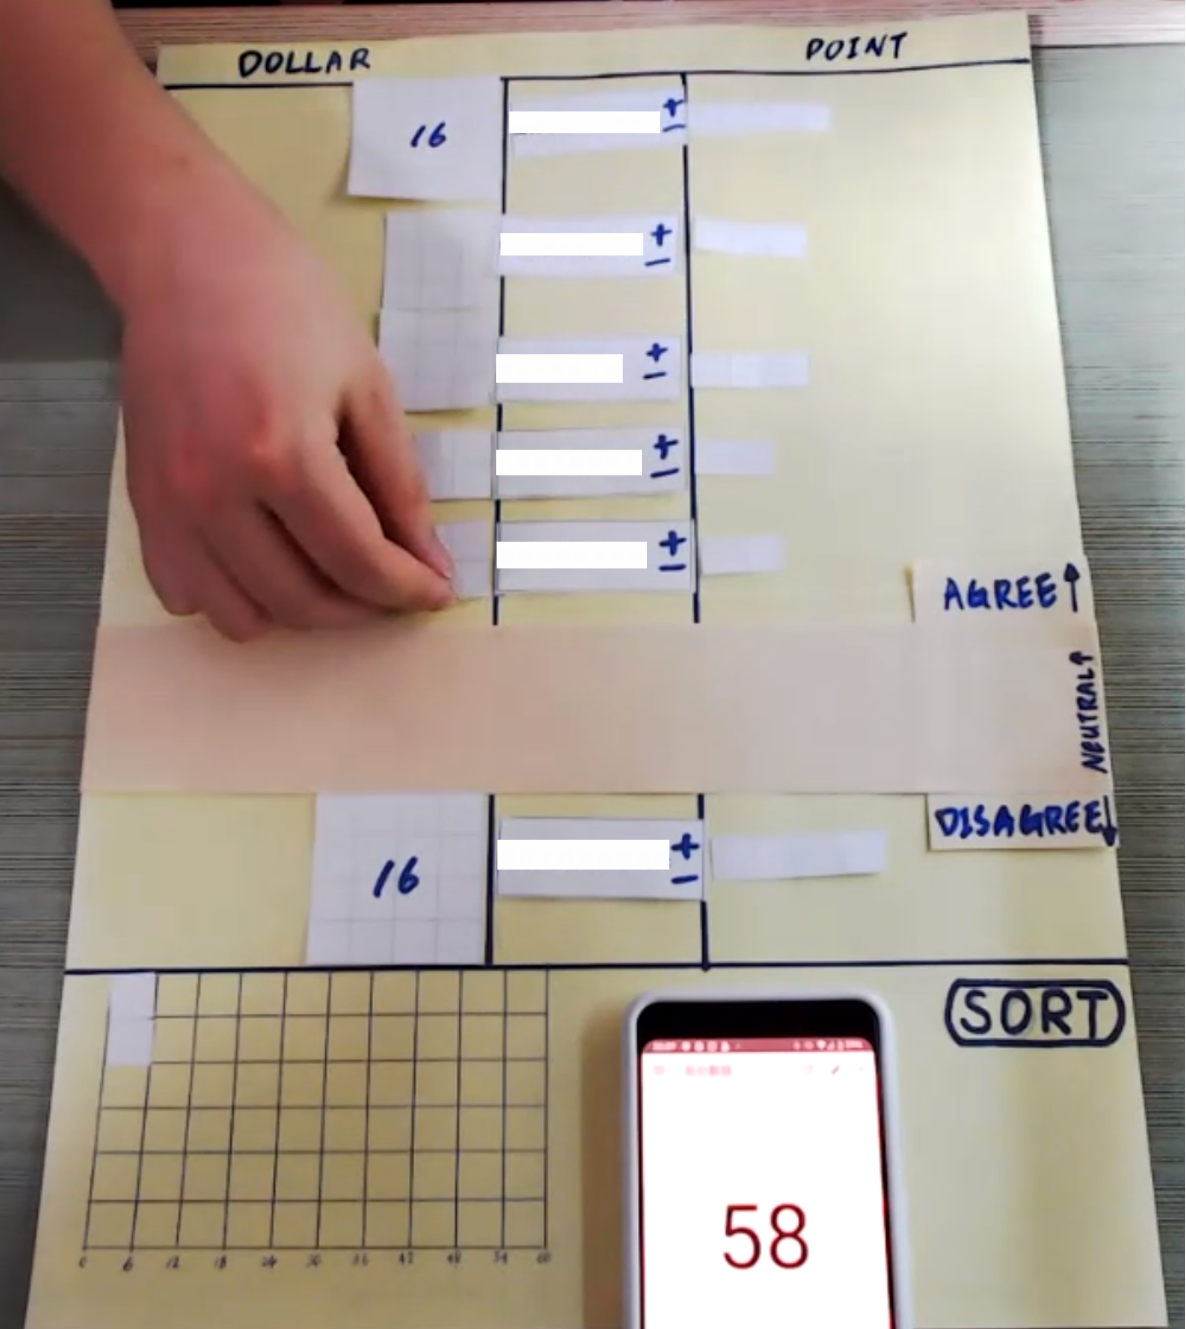
\includegraphics[width=0.77\linewidth]{content/image/prototypes/1_paper_qv_single.png}
        \caption{This paper prototype separates the positive and negative areas with a 'band' at the center. Undecided options are placed inside this band. The cost and the votes on both sides of the interface are denoted by small blocks. The budget is shown in the yellow box below the interface with a numerical counter.}
        \Description{A paper prototype interface where a person's hand is interacting with blocks. The prototype separates positive and negative areas using a wide horizontal band in the center, which holds undecided options. On the left side of the band, a column labeled "Dollar" shows a block marked with the number 16. On the right side, under a column labeled "Point," several rows have small blocks with plus and minus signs, indicating positive and negative areas. At the bottom left, a yellow box with a grid shows the available budget, marked with the number 16. A smartphone in the bottom right corner displays the number 58.}
        \label{fig:vertical_paper}
    \end{subfigure}

    \caption{Initial paper prototypes designed for QS interface.}
    \Description{This figure contains two subfigures showing two different paper prototypes.}
    \label{fig:qv_paper}
\end{figure}

\subsection{Prototype 1: Ranking-Vote}
Our first prototype emerged after various paper prototypes, such as those shown in~\Cref{fig:qv_paper}. Through pre-testing, we observed that participants engaging with QS needed interface support for organizing options and managing their credits. In this study, we decided to focus on the former.

Since participants needed to position options within the interface, and the end result formed a ranked list, we tested whether ranking options before voting would help establish an individual's relative preferences in Prototype 1 (~\Cref{fig:qv_rank}). This prototype allowed respondents to reposition options before voting. However, pre-test respondents rarely moved the options and questioned the necessity of a full ranking, as it did not influence their QS submission. Additionally, many were unaware that the options were draggable. These findings suggest that a full ranking is unnecessary for establishing relative preferences. Therefore, we decided to ask respondents to select a subset of options rather than requiring a full ranking of all options.

\begin{figure}[H]
    \centering
    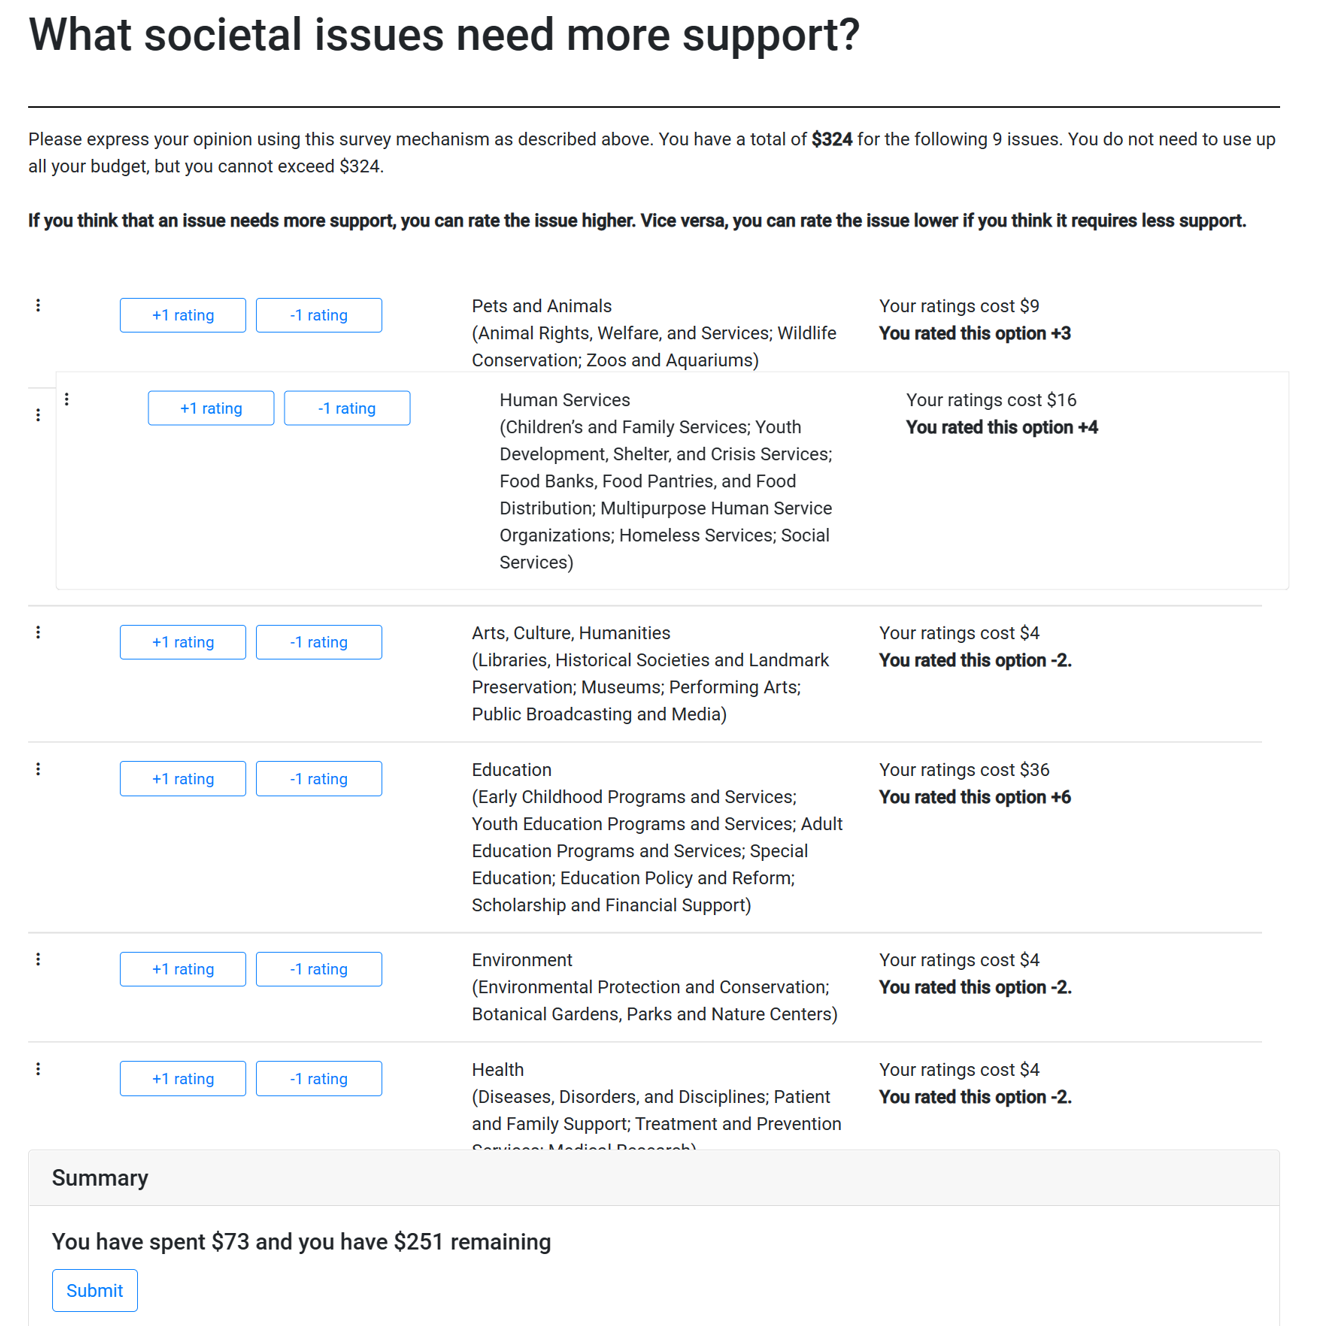
\includegraphics[width=0.43\textwidth, trim={7 7 7 8}, clip]{content/image/prototypes/2_ranking.png}
    \caption{A Ranking-Vote Prototype: This prototype tests whether ranking options prior to voting helps establish an individual's relative preferences. Each option is draggable, allowing users to position it within the full list of options. Votes can be adjusted using the buttons on the left side of the interface, while the vote count and costs are displayed on the right. A summary box remains fixed at the bottom of the screen for easy reference.}
    \Description{A web interface showing a survey titled "What societal issues need more support?" The interface presents several societal issues in a list format, each with buttons labeled "+1 rating" and "-1 rating" to adjust the ratings. For example, the issue "Pets and Animals" shows a rating cost of \$9 with a +3 rating, and "Human Services" shows a rating cost of \$16 with a +4 rating. The remaining issues include Arts, Culture, Humanities, Education, Environment, and Health, each with their respective ratings and costs. At the bottom of the page is a summary box displaying the total spent (\$73) and the remaining balance (\$251). A "Submit" button is positioned below the summary.}
    \label{fig:qv_rank}
    \vspace{-3ex}
\end{figure}

\begin{figure*}[p]
    \centering
    \begin{subfigure}[b]{0.47\textwidth}
        \centering
        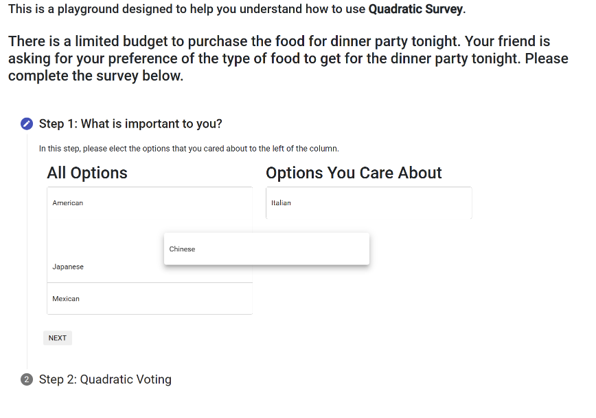
\includegraphics[width=0.95\textwidth]{content/image/prototypes/3.1_selecting.png}
        \caption{Options are dragged and dropped to the 'Option You Care About' box.}
        \Description{A web interface showing the first step of a quadratic voting prototype. The screen is titled "What is important to you?" On the left, under "All Options," a list of food types is displayed, including American, Japanese, and Mexican. One option, "Chinese," is being dragged to the right column labeled "Options You Care About," which already includes "Italian." A "Next" button appears at the bottom of the interface.}

        \label{fig:qv_select_selection}
    \end{subfigure}
    \hfill
    \begin{subfigure}[b]{0.47\textwidth}
        \centering
        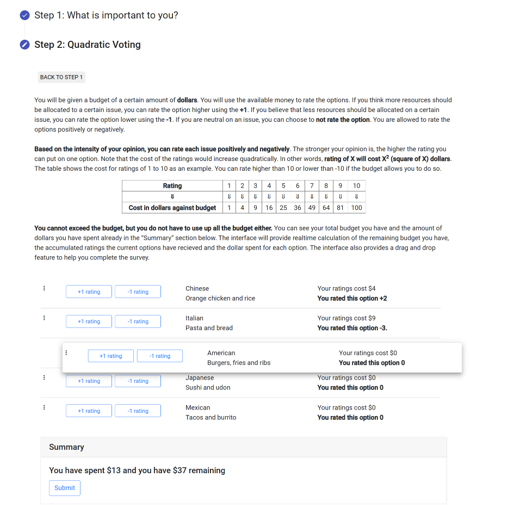
\includegraphics[width=0.9\textwidth]{content/image/prototypes/3.2_selecting_2.png}
        \caption{The previous step collapses showing all voting options.}
        \Description{The second step of a quadratic voting prototype showing a list of food options for voting. The voting interface displays food items such as Chinese, Pasta and bread, and American. Next to each item are "+1 rating" and "-1 rating" buttons for adjusting votes. Each option also shows the cost of votes, and a summary box at the bottom displays the amount spent (\$13) and the remaining balance (\$37).}

        \label{fig:qv_select_vote}
    \end{subfigure}
    \caption{A Select-then-Vote Prototype: The goal of this prototype is to nudge participants to focus on a subset of options to vote, rather than ranking all of them. This prototype introduces a two-step voting process. As shown in Fig.~\ref{fig:qv_select_selection}, the first step involves selecting options for further consideration. Important options are placed at the top of the list for voting shown in Fig.~\ref{fig:qv_select_vote}, but options can be placed anywhere on the list if desired. The rest of the controls follows the previous prototype.}
    \Description{A two-step quadratic voting prototype interface. In the first step (Subfigure 1), users drag and drop food options from a list on the left, such as American and Mexican, to the "Options You Care About" box on the right. In the second step (Subfigure 2), users vote on their selected options by adjusting the ratings using "+1 rating" and "-1 rating" buttons. A summary at the bottom shows the total amount spent and remaining balance.}

    \label{fig:qv_select}
\end{figure*}

\begin{figure*}[p]
    \centering
    \begin{subfigure}[b]{0.45\textwidth}
        \centering
        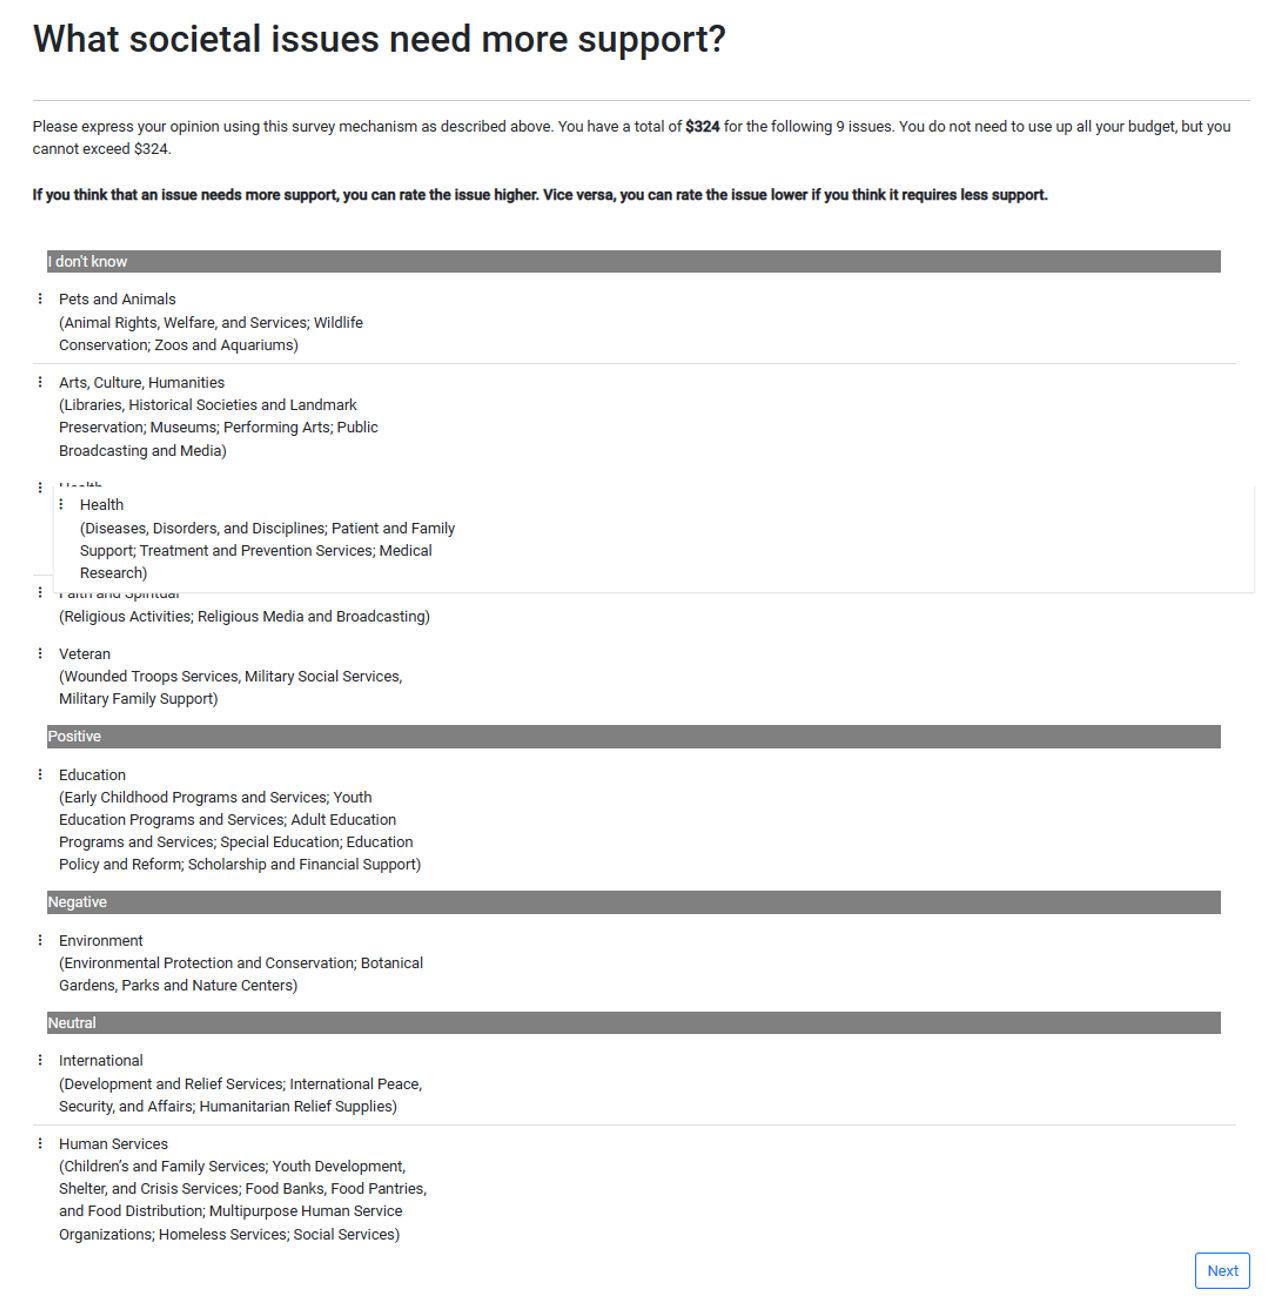
\includegraphics[width=\textwidth]{content/image/prototypes/4.1_grouping.png}
        \caption{The Organization Interface: Options are shown initially in the first bin labeled as `I don't know.' Survey respondents can then drag and drop these options into the latter bins: Lean Positive, Lean Neutral, or Lean Negative. Only the details of each option are shown on this interface.}
        \Description{A web interface displaying a survey titled "What societal issues need more support?" Initially, all options are placed in the first bin labeled "I don't know." The listed options include Pets and Animals, Arts, Culture, Humanities, Health, Veterans, and others. Each option is accompanied by a brief description. Below the "I don't know" bin are three other bins: "Positive," "Negative," and "Neutral." Survey respondents can drag and drop options into these bins based on their preferences. A "Next" button is located at the bottom right corner of the interface.}
        \label{fig:qv_org_p1}
    \end{subfigure}
    \hfill
    \begin{subfigure}[b]{0.45\textwidth}
        \centering
        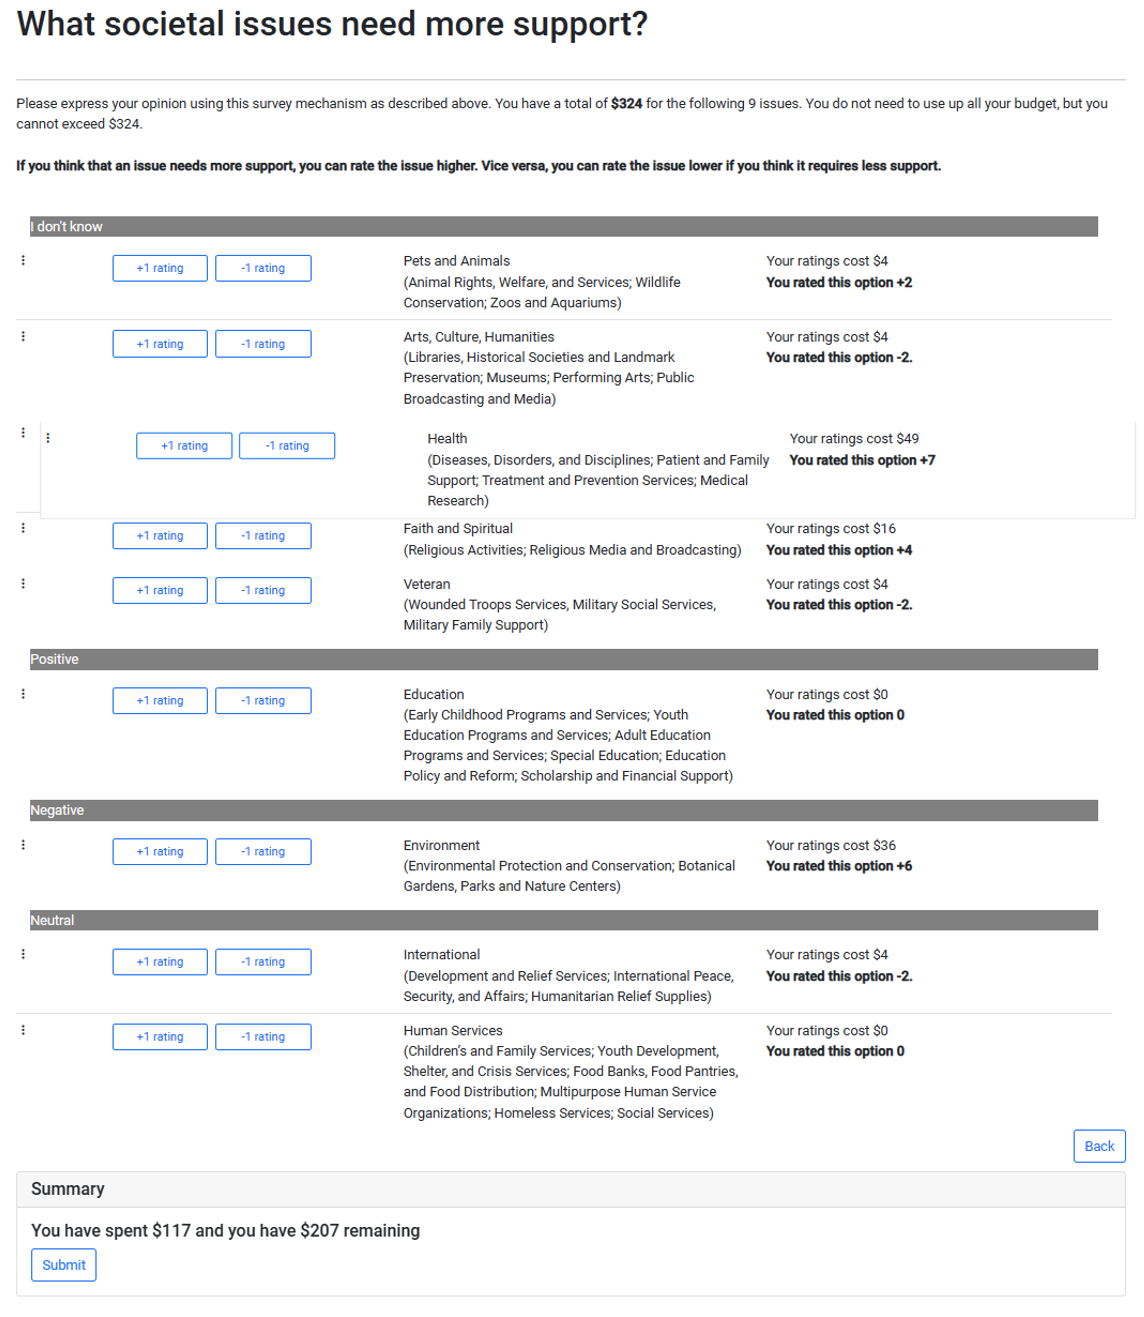
\includegraphics[width=\textwidth]{content/image/prototypes/4.2_grouping_vote.png}
        \caption{The Voting Interface: Voting controls appear on the left side of each option, showing the current votes and associated costs on the right. A budget summary sticks to the bottom of the screen.}
        \Description{A web interface displaying a survey titled "What societal issues need more support?" Each option in the list has voting controls, with "+1 rating" and "-1 rating" buttons appearing on the left side of each issue. The issues are grouped into categories such as "I don't know," "Positive," "Negative," and "Neutral." To the right of each issue, the cost of the rating is shown along with the number of votes cast. For example, "Pets and Animals" has a rating cost of \$4 with a +2 rating, while "Health" has a rating cost of \$49 with a +7 rating. At the bottom of the page, a summary box shows the total amount spent (\$117) and the remaining balance (\$207), with a "Submit" button below it.}

        \label{fig:qv_org_p2}
    \end{subfigure}
    \caption{Organize-then-Vote Prototype: The goal of this prototype is to encourage participants to derive finer grain categories among options before voting. Survey respondents first organize their thoughts into categories and then vote on the options.}
    \Description{The figure shows an Organize-then-Vote prototype with two main steps. In the first step, the left figure, users organize options by dragging and dropping them into different categories: "I don't know," "Positive," "Neutral," or "Negative." In the second step, the right figure, users vote on these organized options using "+1 rating" and "-1 rating" buttons, with voting costs and current ratings displayed. A summary section shows the total spent and remaining budget.}
    \label{fig:qv_org}
\end{figure*}

\subsection{Prototype 2: Select-then-Vote}
Based on feedback from Prototype 1, instead of \textit{allowing} individuals to rank options, Prototype 2 implemented a two-phase process that \textit{intentionally} asks respondents to select options to express opinions before voting. 

As shown in Figure~\ref{fig:qv_select}, survey respondents selected their preferred options (Figure~\ref{fig:qv_select_selection}), and the interface positioned these options at the top of the list for voting (Figure~\ref{fig:qv_select_vote}). We identified several issues during the prototype 2 pretest: many respondents marked most options as 'options they care about,' which undermined the design's purpose. Additionally, the lack of clear distinction between selected and unselected options confused respondents about the necessity of Step 1. Thus, we need a clearer distinction and connection between the two phases to effectively construct relative preferences.

\subsection{Prototype 3: Organize-then-Vote}
Figure~\ref{fig:qv_org} shows the final prototype, which builds on our previous takeaway by introducing finer-grained groupings and establishing a clearer connection between option organization and voting position. Specifically, we provided three categories: Lean Positive, Lean Negative, and Lean Neutral. Initially, respondents see all options listed under a section labeled 'I don't know,' which displays only the option descriptions and not the vote controls. They are then asked to move these options into one of the three categories. On the subsequent page, voting controls and additional information appear for each option, reinforcing the connection between option grouping, position, and voting controls.

Feedback indicated that survey respondents are comfortable with the two-phase organize-then-vote design, demonstrating it as a central strategy for our interface development. However, we identified several areas for enhancement: First, the dragging and dropping mechanism in the organization phase is cumbersome and may inadvertently suggest a ranking process, contrary to our intentions. Second, placing unorganized options at the top of the voting list is counterintuitive. Third, the voting controls are disconnected from the option summaries, dividing attention between the left and right sides of the screen. These insights guided refinements in the final two-phase interface, adhering to the organize-then-vote framework.
